% begin module exponential-function-def
\begin{frame}
\frametitle{(1.5) Exponential Functions}
The function $f(x) = 2^x$ is called an exponential function because the variable $x$ is the exponent.
\begin{columns}[c]
\column{.5\textwidth}
\only<handout:0| -2>{%
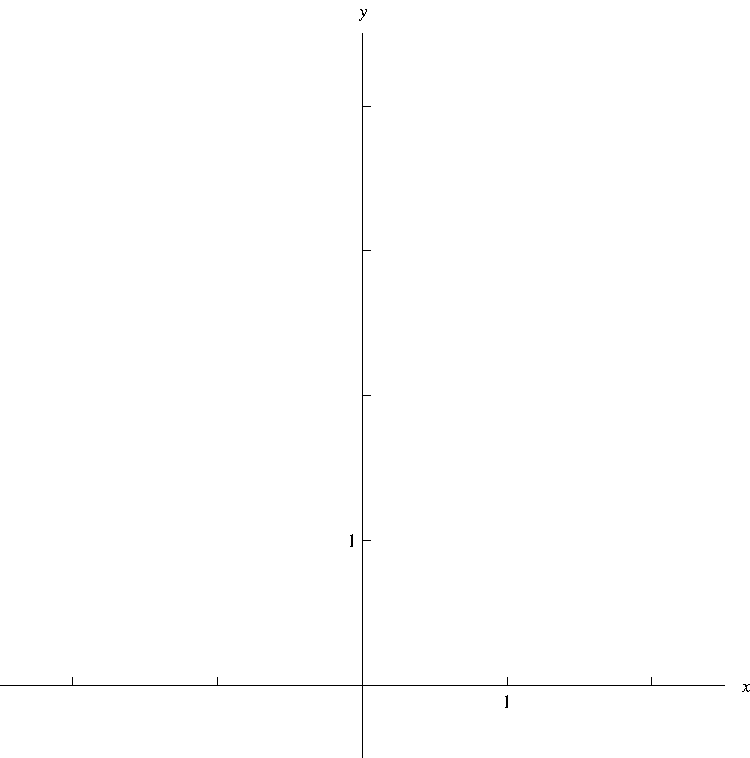
\includegraphics[height=6cm]{exponential-functions/pictures/twoxa.pdf}%
}%
\only<handout:0| 3-4>{%
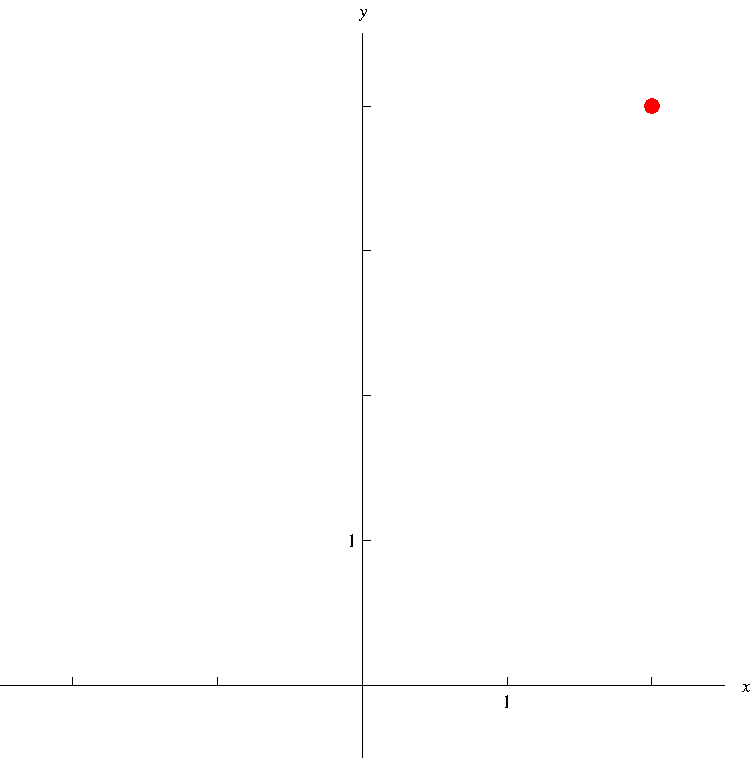
\includegraphics[height=6cm]{exponential-functions/pictures/twoxb.pdf}%
}%
\only<handout:0| 5-6>{%
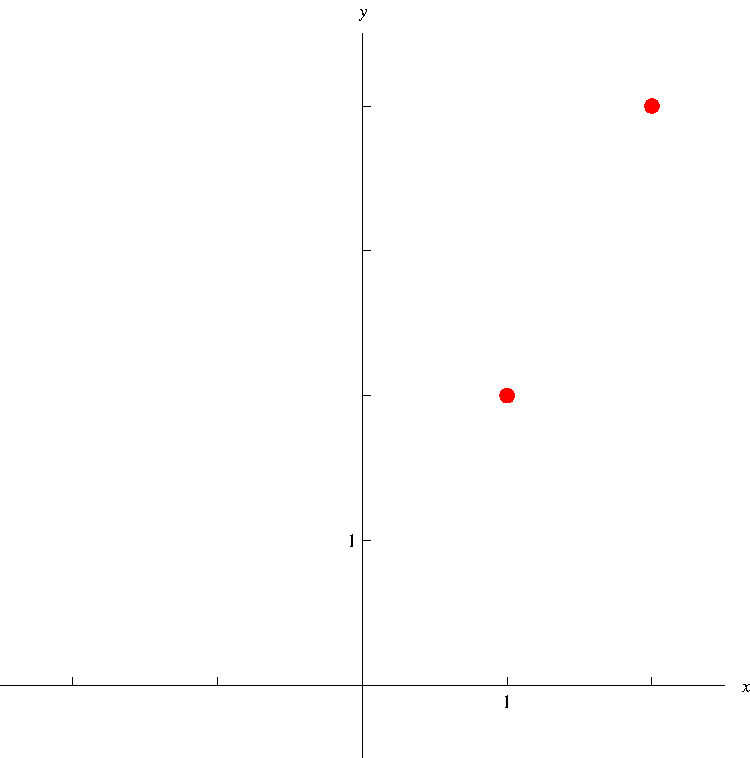
\includegraphics[height=6cm]{exponential-functions/pictures/twoxc.pdf}%
}%
\only<handout:0| 7-8>{%
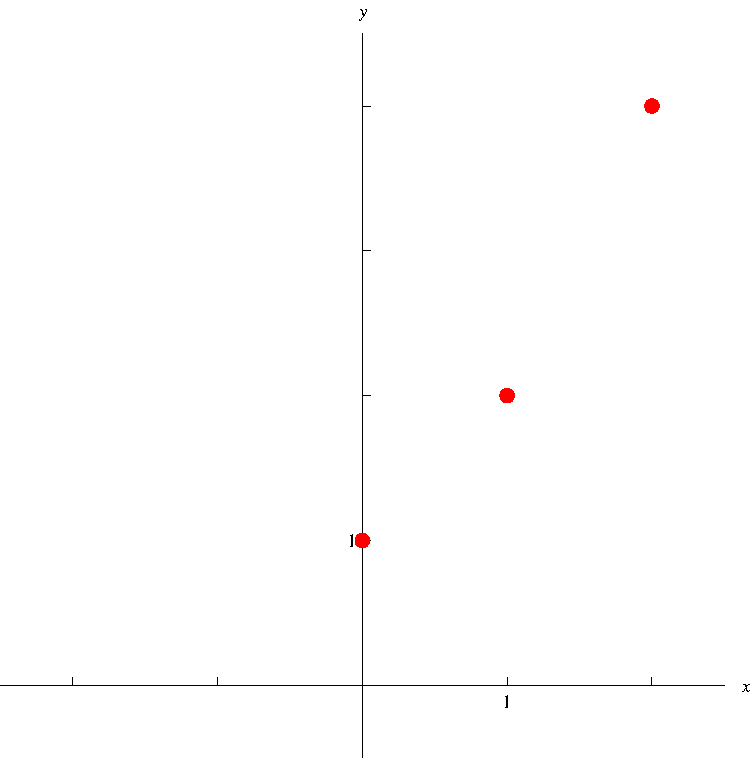
\includegraphics[height=6cm]{exponential-functions/pictures/twoxd.pdf}%
}%
\only<handout:0| 9-10>{%
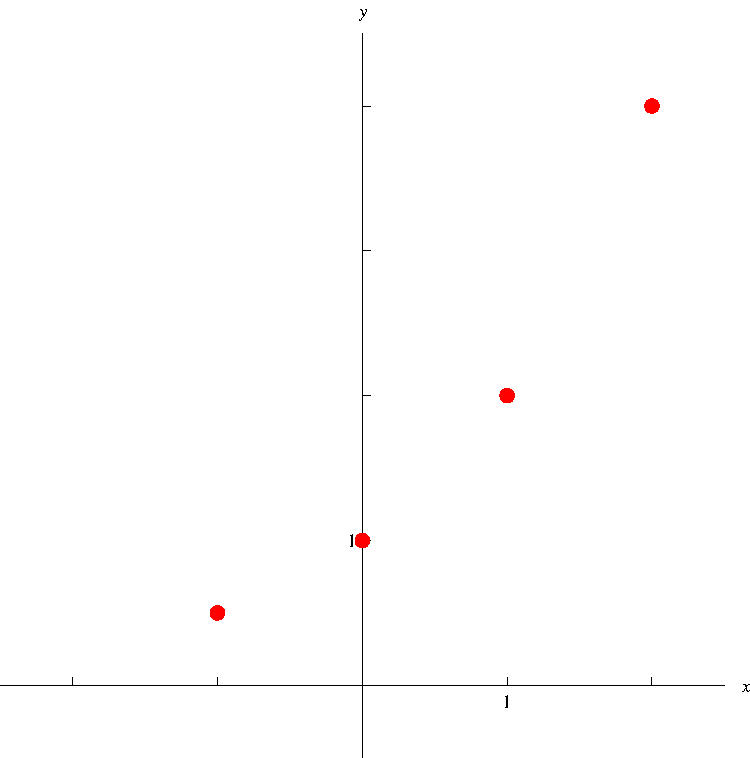
\includegraphics[height=6cm]{exponential-functions/pictures/twoxe.pdf}%
}%
\only<handout:0| 11>{%
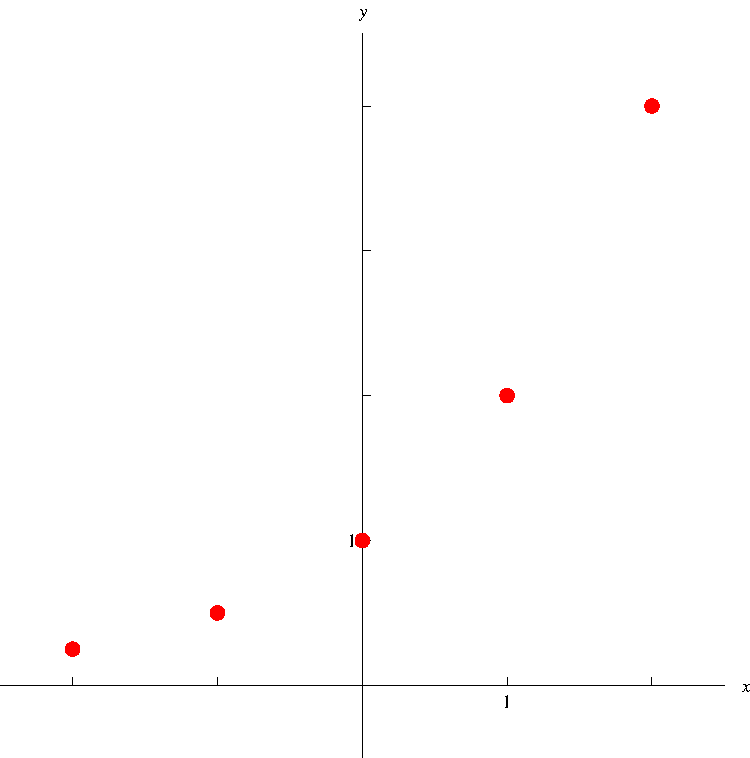
\includegraphics[height=6cm]{exponential-functions/pictures/twoxf.pdf}%
}%
\only<handout:1| 12->{%
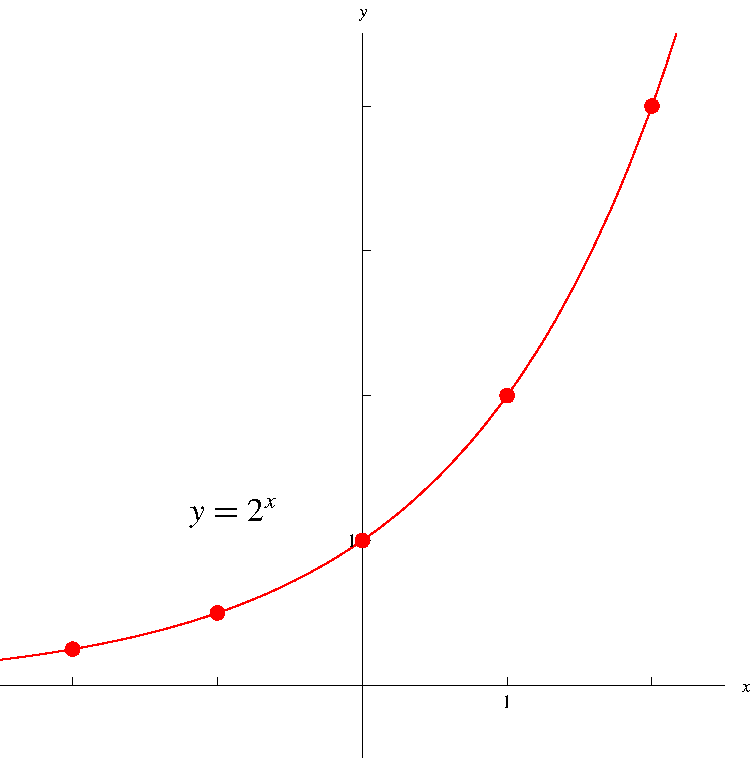
\includegraphics[height=6cm]{exponential-functions/pictures/twoxg.pdf}%
}%
\column{.5\textwidth}
\[
\begin{array}{r|l}
x & y\\
\hline
\alert<handout:0| 2-3>{2} & \alert<handout:0| 3>{\uncover<3->{4}} \\
\alert<handout:0| 4-5>{1} & \alert<handout:0| 5>{\uncover<5->{2}} \\
\alert<handout:0| 6-7>{0} & \alert<handout:0| 7>{\uncover<7->{1}} \\
\alert<handout:0| 8-9>{-1} & \alert<handout:0| 9>{\uncover<9->{1/2}} \\
\alert<handout:0| 10-11>{-2} & \alert<handout:0| 11>{\uncover<11->{1/4}} 
\end{array}
\]
\uncover<13->{
\begin{definition}[Exponential Function]
In general, an exponential function is a function of the form $f(x) = a^x$, where $a$ is a positive constant.
\end{definition}
}
\end{columns}
\end{frame}
% end module exponential-function-def
